

\tikzset{every picture/.style={line width=0.3pt}} %set default line width to 0.75pt        

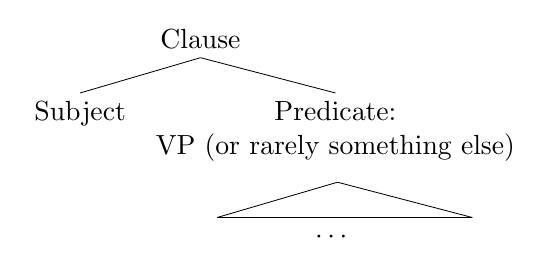
\begin{tikzpicture}[x=0.75pt,y=0.75pt,yscale=-1,xscale=1]
%uncomment if require: \path (0,300); %set diagram left start at 0, and has height of 300

%Straight Lines [id:da9834013734875582] 
\draw    (125,95.81) -- (183,78.81) ;
%Straight Lines [id:da10465096544133767] 
\draw    (248,95.81) -- (183,78.81) ;
%Straight Lines [id:da9284048202068891] 
\draw    (191,155.81) -- (249,138.81) ;
%Straight Lines [id:da46755571549890007] 
\draw    (314,155.81) -- (249,138.81) ;
%Straight Lines [id:da9217356601959923] 
\draw    (191,155.81) -- (314,155.81) ;

% Text Node
\draw (183,75.81) node [anchor=south] [inner sep=0.75pt]   [align=left] {Clause};
% Text Node
\draw (125,98.81) node [anchor=north] [inner sep=0.75pt]   [align=left] {\begin{minipage}[lt]{36.4pt}\setlength\topsep{0pt}
\begin{center}
Subject
\end{center}

\end{minipage}};
% Text Node
\draw (248,98.81) node [anchor=north] [inner sep=0.75pt]   [align=left] {\begin{minipage}[lt]{134.96pt}\setlength\topsep{0pt}
\begin{center}
Predicate:\\VP (or rarely something else)
\end{center}

\end{minipage}};
% Text Node
\draw (237,161.4) node [anchor=north west][inner sep=0.75pt]    {$\cdots $};


\end{tikzpicture}
